\documentclass[11pt,a4paper]{article}
% Portable, journal-proportioned provisional version. See README for the official class status.
\usepackage[T1]{fontenc}
\usepackage[utf8]{inputenc}
\usepackage{lmodern,microtype}
\usepackage{amsmath,amssymb,bm}
\usepackage{graphicx,booktabs,array}
\usepackage[colorlinks=true,citecolor=blue!45!black,urlcolor=blue!45!black,linkcolor=black]{hyperref}
\usepackage{xcolor}
\usepackage{geometry}
\geometry{a4paper,textwidth=145mm,textheight=244mm,centering}
\setlength\parindent{1.15em}
\setlength\parskip{0pt}
\setlength\abovecaptionskip{4pt}
\setlength\belowcaptionskip{3pt}
\setlength\textfloatsep{9pt plus 2pt minus 2pt}
\setlength\intextsep{8pt plus 2pt minus 2pt}
\graphicspath{{figures/}}
\newcommand{\lhmc}{LH$\mu$C}
\newcommand{\sgg}{S_{\gamma\gamma}}
\newcommand{\wgg}{W_{\gamma\gamma}}
\newcommand{\eel}{\mathrm{el}}
\newcommand{\inel}{\mathrm{inel}}
\newcommand{\TeV}{\,\mathrm{TeV}}
\newcommand{\GeV}{\,\mathrm{GeV}}
\newcommand{\fb}{\,\mathrm{fb}}
\newcommand{\pb}{\,\mathrm{pb}}
\renewcommand{\refname}{References}
\begin{document}
\begin{center}
{\Large\bfseries Two-Photon Physics at a Lepton--Proton Collider at CERN\par}
\vspace{7pt}
{\normalsize Hamzeh Khanpour\par}
\vspace{2pt}
{\small Faculty of Physics and Applied Computer Science, AGH University of Krakow,\par
Krak\'ow, Poland\par}
\vspace{6pt}
{\small\itshape Contribution related to the ``Ultra-cold muons for the LHC'' workshop, Krak\'ow, September 2026\par}
\end{center}
\vspace{-4pt}
\begin{abstract}
\noindent
High-energy photon--photon scattering is a complementary component of the physics programme at future CERN lepton--proton facilities. We examine the equivalent-photon description of elastic and proton-dissociative two-photon reactions and discuss their prospects at the Large Hadron--electron Collider (LHeC) and a proposed muon--proton collider (LH$\mu$C). The photon luminosity, rather than the nominal lepton--proton energy alone, determines the rate of a hard two-photon subprocess. Two illustrative precision benchmarks are emphasized: tau-lepton pair production as a probe of electromagnetic dipole interactions, and $W$-boson pair production as a test of the electroweak quartic gauge sector. We distinguish previously studied collider benchmarks from newer, higher-energy muon-beam proposals and discuss how high-invariant-mass distributions may amplify beyond-Standard-Model effects. Loop-induced neutral gauge-boson production, top pairs, charged electroweak states and light-by-light scattering provide additional opportunities. The quantitative interpretation of anomalous-coupling effects requires consistent photon-emission selections, effective-field-theory validity checks and detector-level studies.
\end{abstract}
\vspace{-6pt}
\section{Introduction}
Photon--photon fusion offers a particularly transparent route to the production of electrically charged and electroweakly coupled final states. A relativistic lepton and proton radiate photons, which subsequently undergo a hard collision, $\gamma\gamma\to X$. The radiating particles may remain intact, giving a fully exclusive topology, or the proton may dissociate into a low- or high-mass hadronic system. This separation of electromagnetic emission and the short-distance subprocess underlies the equivalent photon approximation (EPA)~\cite{Budnev1975,Drees1989}.

The proposed Large Hadron--electron Collider (LHeC) combines a lepton beam of order $50\GeV$ with the $7\TeV$ LHC proton beam, yielding $\sqrt{s_{ep}}\simeq1.2\TeV$~\cite{LHeCCDR2012,LHeC2025}. An electron--proton environment is especially attractive for exclusive studies because it has one rather than two colored incoming beams and is expected to have much less event pileup than high-luminosity proton--proton collisions. Neither advantage removes detector inefficiencies, proton dissociation or all soft-interaction uncertainties, but both simplify the experimental interpretation of photon-fusion signatures~\cite{ForthommeDIS2024,ForthommeICHEP2024}.

A complementary LH$\mu$C concept uses energetic positive muons against LHC proton beams. Early two-photon studies employed $E_{\mu}=0.5\TeV$, corresponding to $\sqrt{s_{\mu p}}\simeq3.74\TeV$. The recent proposal of Ref.~\cite{Piotrzkowski2026} emphasizes $1$ and $2\TeV$ muon beams, leading to $\sqrt{s_{\mu p}}\simeq5.3$ and $7.5\TeV$, respectively, with a projected average luminosity approaching $10^{34}\,\mathrm{cm}^{-2}\mathrm{s}^{-1}$. These are machine scenarios: published photon-fusion predictions must be associated with the particular energy and photon selections actually used in each calculation.

We outline the EPA and the energy dependence of its luminosity function, and focus on two physics cases that connect Standard-Model (SM) cross sections with higher-dimensional interactions: $\gamma\gamma\to\tau^+\tau^-$ and $\gamma\gamma\to W^+W^-$. Other charged and neutral final states complete a broader programme in which a high-energy photon spectrum, clean event topology and differential observables are complementary assets.

\section{Theoretical framework for two-photon interactions}
\subsection{Equivalent photon approximation}
For $\ell=e^-$ or $\mu^+$, the generic reaction is $\ell p\to\ell+X+p^{(*)}$. In the quasi-real limit the cross section can be written as a convolution of photon spectra and the elementary photon--photon cross section,
\begin{equation}
\sigma_{\ell p\to\ell Xp^{(*)}} = \int_0^1dy_\ell\int_0^1dy_p\,\Phi_\ell(y_\ell)\Phi_p(y_p)\,\hat\sigma_{\gamma\gamma\to X}(\wgg),
\label{eq:epa}
\end{equation}
where $y_i$ is the fractional energy carried by the photon and $\Phi_i(y_i)=dN_{\gamma/i}/dy_i$. Here $\wgg$ denotes the diphoton invariant mass, with $\wgg^2\simeq y_\ell y_p s_{\ell p}$ for collinear, quasi-real emission. Its natural generalization is
\begin{equation}
\begin{aligned}
\sigma_{\ell p}&=\int_{W_{\rm thr}}^{\sqrt{s_{\ell p}}}dW\,\sgg(W)\,\hat\sigma_{\gamma\gamma\to X}(W),\\
\sgg(W)&=\frac{2W}{s_{\ell p}}\int_{W^2/s_{\ell p}}^1\frac{dy_\ell}{y_\ell}\,\Phi_\ell(y_\ell)\Phi_p\!\left(\frac{W^2}{s_{\ell p}y_\ell}\right).
\end{aligned}
\label{eq:lum}
\end{equation}
Thus $\sgg$ has dimensions of inverse energy, and its integral over $W$ gives a dimensionless effective two-photon luminosity fraction. Equation~(\ref{eq:lum}) is a collinear EPA identity, not an exact statement at arbitrarily high photon virtuality.

\begin{figure}[t]
\centering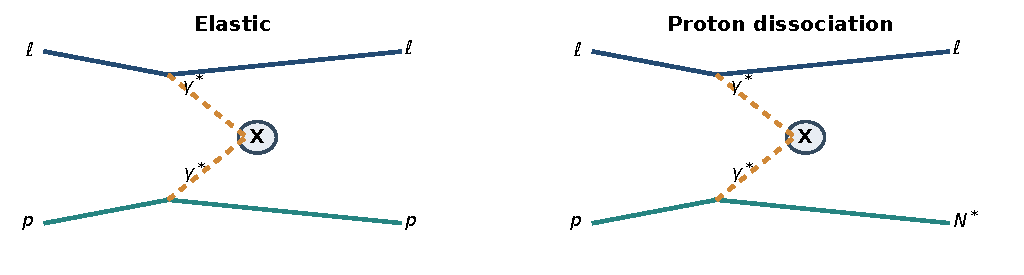
\includegraphics[width=.97\linewidth]{gamma_gamma_topologies.pdf}
\caption{Schematic lepton--proton photon-fusion topologies. The proton remains intact in elastic emission (left) or dissociates into a hadronic state $N^*$ (right). The hard $\gamma\gamma\to X$ subprocess is common to both.}
\label{fig:topologies}
\end{figure}

\subsection{Equivalent-photon spectra and photon virtuality}
For a point-like lepton of mass $m_\ell$, an illustrative virtuality-integrated EPA spectrum is~\cite{Budnev1975}
\begin{equation}
\begin{aligned}
\Phi_\ell(y)&=\frac{\alpha}{2\pi}\left[\frac{1+(1-y)^2}{y}\ln\frac{Q_{\max}^2}{Q_{\min}^2}-\frac{2(1-y)}{y}\left(1-\frac{Q_{\min}^2}{Q_{\max}^2}\right)\right],\\
Q_{\min}^2&\simeq\frac{m_\ell^2y^2}{1-y}.
\end{aligned}
\label{eq:lepton}
\end{equation}
for $Q_{\min}^2<Q_{\max}^2$, with a vanishing flux otherwise. The muon mass increases $Q_{\min}^2$ relative to an electron at fixed $y$: the gain from a muon collider therefore comes from its accessible beam energy and usable phase space, not from a universally larger flux at fixed energy.

For an elastic proton, an often used representation is
\begin{equation}
\Phi_p^{\eel}(y)=\frac{\alpha}{\pi y}\int_{Q_{\min}^2}^{Q_{\max}^2}\frac{dQ^2}{Q^2}\left[(1-y)\left(1-\frac{Q_{\min}^2}{Q^2}\right)F_E(Q^2)+\frac{y^2}{2}F_M(Q^2)\right],
\label{eq:proton}
\end{equation}
where $F_E=(4m_p^2G_E^2+Q^2G_M^2)/(4m_p^2+Q^2)$ and $F_M=G_M^2$ involve the Sachs electromagnetic form factors~\cite{Drees1989}. Here $Q^2=-q^2>0$ denotes the photon virtuality, and the integration bounds must be matched to the tagging or acceptance cuts. For the proton-dissociative channel $p\to\gamma^*+N^*$, the photon spectrum can instead be expressed through measured inclusive electromagnetic structure functions $F_2(x,Q^2)$ and $F_L(x,Q^2)$~\cite{Manohar2016,Manohar2017}. With $M_N$ the dissociation mass, $x=Q_p^2/(M_N^2-m_p^2+Q_p^2)$, so that
\begin{equation}
M_N^2-m_p^2=Q_p^2\left(\frac{1}{x}-1\right).
\label{eq:mn}
\end{equation}
An expanded dissociation phase space can raise the predicted rate, but it changes the final-state topology and increases sensitivity to the structure-function treatment. In particular, an inclusive photon PDF and a proton-tagged elastic flux should not be regarded as interchangeable inputs.

\subsection{Validity of the approximation}
For $Q_\ell^2,Q_p^2\ll W^2$, transverse quasi-real photons dominate and Eqs.~(\ref{eq:epa})--(\ref{eq:lum}) are well motivated. Larger virtualities modify the $\gamma^*\gamma^*$ matrix element, the accessible kinematics and, potentially, photon polarizations. Full virtuality-dependent treatments or matrix-element calculations are then more appropriate. These limitations are particularly relevant in high-mass tails or if very generous virtuality cuts are employed. Keeping the event selection and the virtuality assumptions explicit is necessary for a meaningful comparison between collider options.

\section{Photon--photon luminosity at the LHeC and LH$\mu$C}
Table~\ref{tab:machines} summarizes representative beam configurations. The relation $s_{\ell p}\simeq4E_\ell E_p$ is sufficient for the displayed high-energy values. The $0.5\TeV$ muon scenario was used in earlier phenomenological studies, while the $1$ and $2\TeV$ configurations are highlighted in the newer machine proposal~\cite{Piotrzkowski2026}. A higher $\sqrt{s_{\ell p}}$ permits a harder photon--photon spectrum; however, neither the shape nor normalization of $\sgg$ can be inferred from $\sqrt{s}$ alone.
\begin{table}[h]
\centering\small
\caption{Representative lepton--proton collider configurations. All entries assume a $7\TeV$ proton beam. The figures are nominal machine energies, not measured or guaranteed delivered luminosities.}\label{tab:machines}
\begin{tabular}{@{}lrrl@{}}\toprule
Configuration & $E_\ell$ [GeV] & $\sqrt{s_{\ell p}}$ [TeV] & Interpretation \\ \midrule
LHeC, $e^-p$ & 50 & 1.18 & Reference design \\
LH$\mu$C, $\mu^+p$ & 500 & 3.74 & Earlier baseline \\
LH$\mu$C, $\mu^+p$ & 1000 & 5.29 & Updated proposal \\
LH$\mu$C, $\mu^+p$ & 2000 & 7.48 & Higher-energy proposal \\ \bottomrule
\end{tabular}
\end{table}

For orientation, Fig.~\ref{fig:sgg} shows a \emph{newly evaluated illustrative} EPA example, rather than a replot of the earlier LHeC simulations. It employs Eq.~(\ref{eq:lepton}) with $Q_{\ell,\max}^2=10\GeV^2$ and an elastic proton flux in the Drees--Zeppenfeld dipole approximation~\cite{Drees1989}. In the region of larger $W$, the increase in the kinematic energy scale compensates for the steeper suppression associated with high photon momentum fractions. The quantitative ratio is nevertheless dependent on the allowed $Q^2$ range, proton emission mode and $W$ selection, and the plotted example must not be used as an experimentally validated luminosity forecast.
\begin{figure}[t]
\centering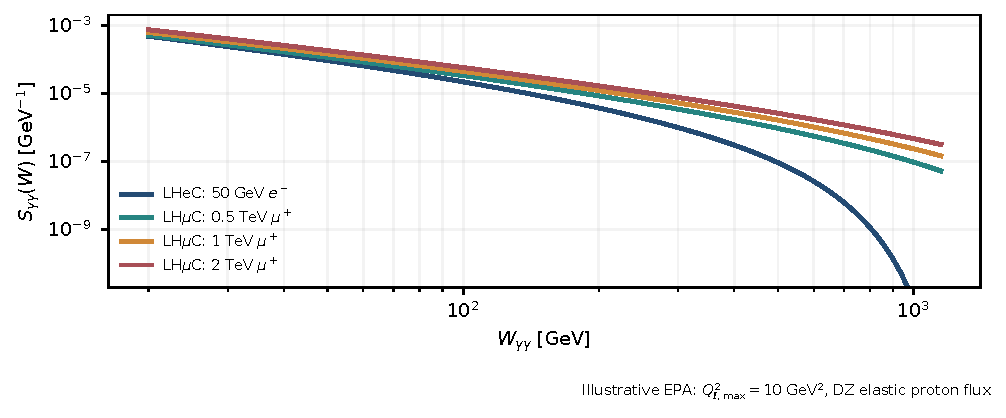
\includegraphics[width=.94\linewidth]{photon_luminosity.pdf}
\caption{Illustrative elastic EPA luminosity spectra obtained from the explicitly stated model in the text (not extracted from the earlier collaborative simulations). The plot is generated reproducibly by the accompanying \texttt{make\_figures.py} script; the $2\TeV$ $\mu^+$ result is a model illustration, not an established LH$\mu$C physics projection.}
\label{fig:sgg}
\end{figure}

\section{Tau-pair production and electromagnetic moments}
\subsection{Standard-Model production}
The tree-level process $\gamma\gamma\to\tau^+\tau^-$ is governed by QED $t$- and $u$-channel tau exchange. The relatively low production threshold makes this channel valuable for photon-luminosity calibration, while the large accessible invariant mass enables a test of the $\gamma\tau\tau$ vertex well above the tau mass. The first observation of photon-induced tau-pair production in $pp$ collisions, together with bounds on tau electromagnetic moments, has already demonstrated the utility of this mechanism~\cite{CMS2024}.

\begin{table}[h]
\centering\small
\caption{Indicative elastic reference cross sections from the prior LHeC/LH$\mu$C analysis. Values are not recalculated in this work; source-level virtuality and acceptance selections require confirmation before publication. The $WW$ entry at $5.3\TeV$ is deliberately left unspecified.}\label{tab:rates}
\begin{tabular}{@{}lcc@{}}\toprule
Machine & $\sigma(\gamma\gamma\to\tau^+\tau^-)$ [pb] & $\sigma(\gamma\gamma\to W^+W^-)$ [pb] \\ \midrule
LHeC ($1.2\TeV$) & $50.40$ & $0.037$ \\
LH$\mu$C ($3.7\TeV$) & $58.5$ & $0.166$ \\
LH$\mu$C ($5.3\TeV$) & $70.3$ & --- \\ \bottomrule
\end{tabular}
\end{table}

The collaborative benchmark values collected in Table~\ref{tab:rates} illustrate a modest increase in the total elastic tau-pair rate as the muon beam energy is raised. Since the underlying acceptance and virtuality definitions could not be recovered here in a machine-readable form, these numbers are treated as \emph{indicative reference inputs}, not independently reproduced predictions; they are intentionally not combined with the separate illustrative flux calculation of Fig.~\ref{fig:sgg}. The key physical observation is more robust than any single integral: more energetic photon--photon collisions extend the measurable $M_{\tau\tau}$ distribution beyond a low-mass dominated inclusive sample.

\subsection{Dipole interactions and their EFT interpretation}
A convenient on-shell description of non-standard tau electromagnetic interactions uses
\begin{equation}
\mathcal L_{\tau\tau\gamma}^{\rm dip}=\frac{e\,\delta a_\tau}{4m_\tau}\,\bar\tau\sigma^{\mu\nu}\tau F_{\mu\nu}-\frac{i\,d_\tau}{2}\,\bar\tau\sigma^{\mu\nu}\gamma_5\tau F_{\mu\nu},
\label{eq:dipole}
\end{equation}
where $\delta a_\tau$ denotes the deviation from the SM magnetic moment and $d_\tau$ is the electric dipole moment; the sign conventions are conventional and must be kept fixed when matching amplitudes. The magnetic term is CP even, whereas the electric term violates CP. At scales above electroweak symmetry breaking, the corresponding new-physics interactions may be embedded in gauge-invariant dimension-six SMEFT operators,
\begin{equation}
\mathcal O_{eB}^{33}=(\bar L_3\sigma^{\mu\nu}\tau_R)H B_{\mu\nu},\qquad \mathcal O_{eW}^{33}=(\bar L_3\sigma^{\mu\nu}\tau_R)\sigma^I H W^I_{\mu\nu},
\label{eq:tauops}
\end{equation}
with $\Delta\mathcal L=(C_{eB}^{33}\mathcal O_{eB}^{33}+C_{eW}^{33}\mathcal O_{eW}^{33})/\Lambda^2+\mathrm{h.c.}$. The physical photon coupling depends on the weak mixing angle and on the real and imaginary parts of the Wilson-coefficient combination. The exact numerical matching should follow the normalization chosen for the SU(2) generators and the dipole vertex.

\subsection{High-mass distributions and sensitivity}
The amplitude may be organized schematically as $\mathcal M=\mathcal M_{\rm SM}+\delta a_\tau\mathcal M_a+d_\tau\mathcal M_d$. Consequently a differential distribution contains interference and higher-order dipole terms, while the CP-odd interference may vanish in sufficiently inclusive CP-even observables. The behavior of $d\sigma/dM_{\tau\tau}$, rather than only the integrated cross section, can therefore improve the separation of anomalous scenarios from the SM. This enhancement must be weighed against the rapid decrease in photon luminosity and the efficiency of reconstructing visible tau decays with escaping neutrinos.

Earlier exploratory plots used $\delta a_\tau=0.008$, whereas an updated study considered $\delta a_\tau=5\times10^{-4}$. Because the original numerical files and curve definitions are not available in the present portable package, we do not reproduce or relabel the corresponding distributions. A genuine exclusion analysis would need binned event yields, backgrounds, systematic uncertainties, correlations and an explicit treatment of the dipole operator's range of validity. It is therefore more accurate here to identify the high-$M_{\tau\tau}$ region as a promising \emph{observable} than to advertise a new confidence-level reach.

\section{$W$-boson pairs and anomalous quartic gauge couplings}
\subsection{Standard-Model $\gamma\gamma\to W^+W^-$}
At leading order $\gamma\gamma\to W^+W^-$ proceeds through charged-$W$ exchange in the $t$ and $u$ channels, together with the four-point $\gamma\gamma W^+W^-$ vertex. Gauge invariance ties these amplitudes together. Unlike massive charged scalar or fermion-pair production, the unpolarized high-energy vector-pair subprocess retains a sizable rate, making it an unusually productive probe of the electroweak gauge sector~\cite{ForthommeICHEP2024}. Its threshold is $W_{\rm thr}=2m_W$, substantially higher than for tau pairs.

For the elastic benchmarks collected in Table~\ref{tab:rates}, the $W$-pair cross section at the LH$\mu$C baseline exceeds the LHeC reference value by a factor of approximately $4.5$. Assuming, purely for illustration, an integrated luminosity of $250\fb^{-1}$ in each configuration, the corresponding produced pair counts are $9.25\times10^3$ and $4.15\times10^4$, respectively, before $W$ decays and experimental effects. These benchmarks have not been re-simulated for this proceeding. They illustrate the difference between the comparatively abundant $W$-pair channel and genuinely rare high-mass final states; they do not establish measurable yields without detector-level reconstruction.

\subsection{Dimension-eight quartic interactions}
Anomalous quartic gauge couplings (aQGCs) are conveniently parameterized in a linearly realized electroweak EFT using higher-dimensional operators. A generic representation is
\begin{equation}
\mathcal L_{\rm EFT}=\mathcal L_{\rm SM}+\sum_i\frac{f_i}{\Lambda^4}\mathcal O_i^{(8)}+\cdots,\qquad \sigma=\sigma_{\rm SM}+\sum_i\frac{f_i}{\Lambda^4}\sigma_{{\rm int},i}+\sum_{ij}\frac{f_if_j}{\Lambda^8}\sigma_{{\rm quad},ij}.
\label{eq:aqgc}
\end{equation}
The commonly used $S$, $M$ and $T$ operator families organize contributions involving covariant Higgs derivatives and electroweak field strengths~\cite{Eboli2006,Eboli2016}. For example, in one standard convention $\mathcal O_{M2}=(B_{\mu\nu}B^{\mu\nu})[(D_\beta H)^\dagger D^\beta H]$. A benchmark such as $f_{M2}/\Lambda^4=1\TeV^{-4}$ changes the amplitude, but is \emph{not} by itself an experimental constraint. Equation~(\ref{eq:aqgc}) also makes clear that large positive high-mass deviations can be dominated by the quadratic EFT term, potentially in a regime where the truncation becomes unreliable.

\subsection{Comparison and EFT domain of validity}
The principal sensitivity of $\gamma\gamma\to WW$ to anomalous contributions occurs in high-$M_{WW}$ bins, where increased hard-scattering energy may offset declining photon luminosity. A collider-to-collider comparison must hold the EFT coefficients, final-state acceptance, photon virtuality cuts and proton-emission topology fixed. In particular, the original LH$\mu$C aQGC distribution used a $5.3\TeV$ collider configuration, while the elastic SM cross-section number just quoted corresponds to $3.7\TeV$; one must not mix them into a single numerical limit. Furthermore, an LHC proton--proton comparison is affected by proton survival probabilities, pileup and tagging conditions that have no simple counterpart in $\ell p$ scattering.

An experimentally interpretable analysis would report the selected reconstructed final state, detector response, background template, correlated uncertainties and treatment of parameter degeneracies. It would also specify an energy domain such that the operator expansion remains controlled. A visible ratio $[d\sigma/dM_{WW}]_{\rm EFT}/[d\sigma/dM_{WW}]_{\rm SM}$ signals a potentially discriminating observable; it is not equivalent to a detector-level 95\% confidence interval. This distinction is central when comparing upgraded LH$\mu$C energies with earlier baseline studies.

\section{Additional Standard-Model and BSM opportunities}
Beyond tau and $W$ pairs, several photon-fusion processes become especially interesting as the accessible diphoton mass increases. The neutral final state $\gamma\gamma\to ZZ$ occurs at one loop in the SM, so an anomalous neutral quartic interaction can have a distinctive influence on the high-mass region. The process $\gamma\gamma\to t\bar t$ provides an electromagnetic channel for the heaviest SM fermion, sensitive in principle to its photon vertex; because its threshold is near $2m_t$, the rate is strongly dependent on the tail of $\sgg$ and must be distinguished from the much larger $\gamma g$ photoproduction channel.

Charged electroweak states provide further threshold benchmarks. Higgsino-like charginos and charged sleptons can be produced through $\gamma\gamma\to\widetilde H^+\widetilde H^-$ and $\gamma\gamma\to\widetilde\ell^+\widetilde\ell^-$. At fixed electric charge and mass the leading photon coupling is constrained, while spin determines the detailed threshold and angular behavior. Compressed spectra are challenging because visible decay products may be soft and missing-momentum signatures depend on precise event reconstruction. Existing LHC searches already constrain portions of this parameter space, so a lepton--hadron measurement would be complementary rather than automatically superior. Figure~\ref{fig:thresholds} records the simple kinematic scales without implying detectability.

\begin{figure}[t]
\centering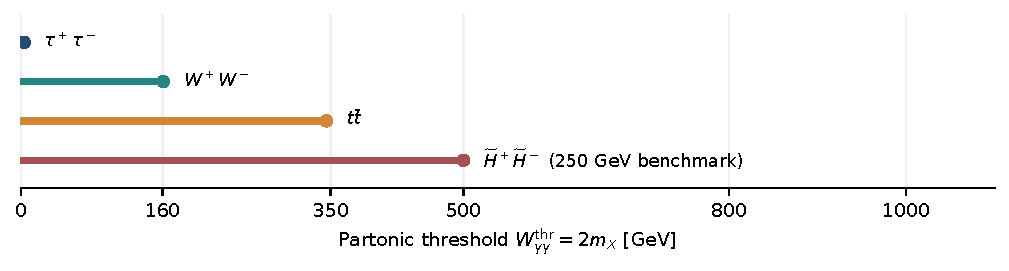
\includegraphics[width=.9\linewidth]{heavy_thresholds.pdf}
\caption{Pair-production thresholds for selected final states, using reference masses. The charged-higgsino mass of $250\GeV$ is an illustrative BSM benchmark; the diagram displays only $W_{\gamma\gamma}\ge 2m_X$ and does not represent cross sections or exclusions.}
\label{fig:thresholds}
\end{figure}

Finally, $\gamma\gamma\to\gamma\gamma$ and the loop-induced single-Higgs process $\gamma\gamma\to H$ probe charged virtual particles through loop amplitudes. Their intrinsic rarity makes the control of exclusive selections, photon spectra and backgrounds especially important. These channels broaden the physics case without altering the priority of higher-statistics tau and $W$-pair studies.

\section{Experimental considerations and future prospects}
A useful photon-fusion analysis must define the outgoing-lepton acceptance, central-system reconstruction and proton final state simultaneously. Elastic channels may exploit near-beam proton tagging, large rapidity gaps, small transverse-momentum imbalance and acoplanarity, while dissociative channels demand either explicit hadronic reconstruction or a carefully modelled inclusive treatment. Tau decays introduce neutrinos; $W$ reconstruction entails branching fractions and combinatorial or missing-energy ambiguities; and charged new-particle signals may be acceptance-limited. These effects are not contained in a generator-level EPA integral.

The machine--detector interface for the LH$\mu$C is still under development~\cite{Piotrzkowski2026}. Quantitative studies must account for muon-beam-related backgrounds, beam optics and tagging acceptance. Future work should therefore combine validated quasi-real photon fluxes with exact matrix elements where required, detector simulations, realistic delivered luminosity assumptions, and statistical fits respecting EFT power counting. In particular, new luminosity and full-process calculations at $5.3$ and $7.5\TeV$ are needed before extrapolating the results obtained for the earlier $3.7\TeV$ scenario.

\section{Summary and conclusions}
High-energy photon fusion offers a complementary electroweak and BSM programme at future CERN lepton--proton colliders. The EPA organizes the connection between the beam-dependent photon fluxes and the hard $\gamma\gamma$ subprocess, while elastic and dissociative proton emission must remain distinct. The LH$\mu$C's higher attainable beam energy creates opportunities in the hard-photon tail, especially for $W$ pairs and heavier states. Tau-pair spectra and quartic-gauge observables furnish well-motivated probes of anomalous interactions, but generator-level shape differences must not be confused with exclusion limits. Consistent kinematic selections, reliable photon emission models, detector response and EFT validity checks are indispensable for the next generation of sensitivity projections.

\bibliographystyle{unsrt}
\bibliography{references}
\end{document}
